%% Revised manuscript prepared for the IEEE Transactions on Intelligent
%% Transportation Systems, using the official IEEEtran class (v1.8b, CTAN).
%%
%% This file is generated from ../main.tex: the body text is carried over
%% unchanged, and only the front matter, the class-specific commands and the
%% bibliography style are adapted to IEEEtran.

\documentclass[journal]{IEEEtran}

\usepackage[numbers,sort&compress]{natbib}
\usepackage{graphicx}
\usepackage{amsmath}
\usepackage{amssymb}
\usepackage{booktabs}
\usepackage{siunitx}
\usepackage{array}
\usepackage[caption=false]{subfig}
\usepackage{algorithm}
\usepackage{algpseudocode}
\usepackage{enumitem}
\usepackage{url}
\usepackage[hidelinks]{hyperref}

% Display and float spacing tightened to IEEE practice; the two-column layout
% is far more sensitive to these skips than the single-column Elsevier one.
\setlength{\abovedisplayskip}{4pt plus 2pt minus 2pt}
\setlength{\belowdisplayskip}{4pt plus 2pt minus 2pt}
\setlength{\abovedisplayshortskip}{2pt plus 1pt minus 1pt}
\setlength{\belowdisplayshortskip}{2pt plus 1pt minus 1pt}
\setlength{\textfloatsep}{8pt plus 2pt minus 2pt}
\setlength{\floatsep}{8pt plus 2pt minus 2pt}
\setlength{\intextsep}{8pt plus 2pt minus 2pt}
\setlength{\dbltextfloatsep}{8pt plus 2pt minus 2pt}
\setlength{\dblfloatsep}{8pt plus 2pt minus 2pt}
\setlist{nosep,leftmargin=*}

% Let floats occupy more of a column before a float page is started, so the
% two-column layout does not leave large gaps around the wide tables.
\renewcommand{\topfraction}{0.92}
\renewcommand{\bottomfraction}{0.7}
\renewcommand{\dbltopfraction}{0.92}
\renewcommand{\textfraction}{0.07}
\renewcommand{\floatpagefraction}{0.8}
\renewcommand{\dblfloatpagefraction}{0.8}

% IEEEtran does not define these cas-sc niceties; the body uses none of them,
% but keeping the hyperref colours matches the Elsevier version.
\hypersetup{
    colorlinks = true,
    citecolor = cyan,
    linkcolor = cyan,
    urlcolor = cyan,
    bookmarksopen = true,
    filecolor = cyan
}

\begin{document}

\title{Learning to Route Electric Trucks Under Operational Uncertainty}

% Author block for the non-anonymous version; the submitted revision is
% anonymized, matching ../main.tex.
% \author{Stavros~Orfanoudakis,~Ziyan~Li,~Ruixiao~Yang,~Nikolay~Aristov,
%         Pedro~P.~Vergara,~Chuchu~Fan,~and~Elenna~Dugundji
% \thanks{S. Orfanoudakis and P. P. Vergara are with the Intelligent Electrical
% Power Grids group, Delft University of Technology, Delft, The Netherlands
% (e-mail: s.orfanoudakis@tudelft.nl).}
% \thanks{S. Orfanoudakis, Z. Li, N. Aristov and E. Dugundji are with the Center
% for Transportation and Logistics, Massachusetts Institute of Technology,
% Cambridge, MA, USA.}
% \thanks{R. Yang and C. Fan are with the Department of Aeronautics and
% Astronautics, Massachusetts Institute of Technology, Cambridge, MA, USA.}}
\author{Anonymous authors}

\markboth{IEEE Transactions on Intelligent Transportation Systems}%
{Anonymous authors: Learning to Route Electric Trucks Under Operational Uncertainty}

\maketitle

\begin{abstract}
Electric truck operations require routing decisions that remain feasible under limited battery range, long charging times, travel and energy consumption, and competition for shared charging infrastructure. These features make electric truck routing a coupled logistics and energy problem, limiting the practicality of heuristic methods at scale. This paper proposes a learning-based framework for stochastic electric truck routing under charging constraints and operational uncertainty. The problem, solved by Reinforcement Learning, is formulated as an event-driven semi-Markov decision process with shared charging resources, stochastic travel and energy requirements, and realistic nonlinear fast-charging behavior. To support learning in this setting, a graph-based representation of system state and feasible decisions is introduced, together with a rule-based action mask that restricts policies to operationally admissible actions. An event-driven simulation environment is developed on this formulation, supporting both Reinforcement Learning and benchmarking against heuristic and mathematical programming baselines. Computational experiments across a range of fleet sizes show that the proposed learning-based algorithm consistently outperforms baselines and attains performance close to optimization benchmarks in many settings, while preserving high success rates under charging congestion and uncertainty.
\end{abstract}

\begin{IEEEkeywords}
Reinforcement Learning, Electric Truck Routing, Freight Transportation, Graph Neural Networks, Stochastic Optimization, Vehicle Routing
\end{IEEEkeywords}

\IEEEpeerreviewmaketitle

\section{Introduction}

The electrification of transportation is transforming mobility and logistics systems by creating new opportunities to reduce emissions, improve energy efficiency, and lower dependence on fossil fuels~\cite{ZHANG2022103152}. The resulting coupling between routing and charging is not unique to freight: electric bus fleets must fit charging around fixed timetables under nonlinear charging dynamics and battery degradation~\cite{jin2024buses}, and electric ride-hailing fleets must trade passenger service off against recharging detours~\cite{shi2020ridehailing}. Freight operations sharpen the problem further, because delivery time windows and payload-dependent energy use leave less slack to absorb a mistimed charge, and because electric trucks operate under limited driving range, long charging times, and uneven charging infrastructure, making charging a central component of route planning rather than a secondary consideration~\cite{KUCUKOGLU2021107650}. As a result, electric truck routing becomes a coupled logistics and energy management problem in which route feasibility and service performance depend not only on delivery sequences~\cite{osti_1615213}, but also on when, where, and how vehicles charge, especially in fleet settings with shared and capacity-constrained charging resources~\cite{BRAGIN2024104494}. 

The electric truck fleet routing problem (eTFRP)~\cite{ziyan2025} has evolved from an extension of the vehicle routing problem (VRP) and electric VRP (eVRP) into a distinct research stream centered on the operational realities of electrified freight~\cite{cataldo_2023}. Optimization-based methods provide its main analytical foundation, embedding charging decisions, uncertainty, and energy-feasibility constraints directly into mathematical models. This line includes stochastic formulations with simplified charging curves~\cite{SPINELLI2026105480}, robust models for heavy-duty electric trucks under uncertain energy consumption~\cite{AMIRI2023109108}, and conic mixed-integer programs capturing richer physical drivers of energy use~\cite{WANG2024123407}. These approaches offer interpretability and disciplined feasibility control, but their computational requirement grows rapidly with fleet size, uncertainty, and modeling realism~\cite{lara_electric_2020}. Metaheuristics such as variable-neighborhood search~\cite{euchi_hybrid_2023}, memetic~\cite{dong_dynamic_2023}, and ant-colony-based methods~\cite{9409782} scale better in practice, although their performance depends on instance structure and parameter tuning and is harder to characterize under uncertainty.

In parallel, Reinforcement Learning (RL) has emerged as a promising direction~\cite{evgnn} because it searches across instances during training and infers rapidly at deployment~\citep{kool2018attention}. Attention-based policies with improved rollout and symmetry-based training perform well on classical routing problems without hand-crafted search rules~\citep{yang2025neural}, and these ideas have been extended to charging-aware, stochastic, and safety-aware electric vehicle routing~\cite{BASSO2022102496}. However, much of this literature remains closer to simple eVRP settings than to fleet-level electric truck operations with shared charging resources, traffic congestion, and truck-specific constraints~\citep{lin2025}. Learning-based approaches also rarely embed explicit feasibility control, and cross-family comparisons are difficult to interpret because they rest on different assumptions about uncertainty, charging behavior, and temporal dynamics~\cite{lin2022}. 

% These gaps point to a clear need for methods that retain the operational realism of electric truck routing while remaining scalable enough for repeated, time-sensitive decision making. In response, this paper develops a truck-oriented and learning-compatible framework for the eTFRP under charging constraints and uncertainty. We formulate the problem in a way that explicitly captures fleet-level interactions through shared charging infrastructure, stochastic travel and energy conditions, and realistic charging behavior, while preserving the structure needed for sequential decision making. On this basis, we introduce GraphPPO, a graph neural network (GNN)-based~\cite{kipf} RL approach that combines a structured state--action representation with an explicit state-based feasibility action mask, allowing routing and charging decisions to be learned without discarding the operational constraints that define the problem. To assess the advantages and the limitations of GraphPPO, we further place it within a common simulation and benchmarking environment that enables direct comparison with heuristic and optimization-based methods under consistent assumptions.

% More specifically, the paper contributions can be summarized as follows:
% \begin{itemize}
%     \item Formulate the eVRP and eTFRP as event-driven semi-Markov decision problems with shared charging resources, stochastic travel and energy consumption, and realistic charging behavior, thereby moving beyond simplified single-vehicle eVRP abstractions toward a truck-oriented realistic operational setting.

%     \item Introduce a graph-based state and action representation, together with a state-based action feasibility mask, that captures interactions among trucks, deliveries, and charging infrastructure while restricting decisions to operationally admissible actions.

%     \item Propose {GraphPPO}, a graph-based actor--critic RL method that operates on the proposed formulation and is designed to learn routing and charging decisions under fleet-level coupling, uncertainty, and variable action spaces.    

%     \item Develop a complete event-driven simulation and benchmarking simulator using real transportation networks from California, together with an extensive computational study, that evaluates not only the effectiveness of the proposed method but also its limits, including scalability relative to mathematical programming baselines and performance in settings where nonlinear charging curves and time-dependent effects weaken standard classical assumptions.
% \end{itemize}

These gaps point to a clear need for methods that retain the operational realism of electric truck routing while remaining scalable enough for repeated, time-sensitive decision making. In response, this paper develops a truck-oriented and learning-compatible framework\footnote{The project code will be open-sourced upon publication.}
% \footnote{The project repository is available at \url{https://github.com/StavrosOrf/eTruckRouting}.}
for the eTFRP under charging constraints and uncertainty. The problem is formulated to explicitly capture fleet-level interactions through shared charging infrastructure, stochastic travel and energy conditions, and realistic charging behavior, while preserving the structure needed for sequential decision-making. On this basis, Graph Proximal Policy Optimization (GraphPPO) is introduced as a graph neural network (GNN)-based~\cite{kipf} RL approach that combines a structured state--action representation with an explicit state-based feasibility action mask, allowing routing and charging decisions to be learned without discarding the operational constraints that define the problem. To assess both the strengths and the limitations of GraphPPO, a common simulation and benchmarking environment is further developed for direct comparison with heuristic and optimization-based methods under consistent assumptions.

More specifically, the paper's contributions can be summarized as follows:
\begin{itemize}
    \item The eVRP and eTFRP are formulated as event-driven semi-Markov decision processes with shared charging resources, stochastic travel and energy consumption, and nonlinear charging, moving beyond simplified abstractions toward a truck-oriented operational setting.

    \item A graph-based state and action representation is introduced together with a state-based action feasibility mask, so that interactions among trucks, deliveries, and charging infrastructure are encoded explicitly while decisions remain restricted to operationally admissible actions.

    \item GraphPPO is proposed as a graph-based actor--critic RL method for routing and charging under fleet-level coupling, uncertainty, and variable action spaces, maintaining near-benchmark performance as problem size increases and obtaining stronger reliability and scalability than the generic PPO and MaskPPO baselines.

    \item A complete event-driven simulation and benchmarking environment is developed on real California transportation networks, with a computational study of scalability, robustness, and transferability against heuristic and mathematical programming baselines. It shows competitiveness in large congested fleets, parity with a validated exact planner on fleet travel time when assignment and sequencing are also decided, and transfer that degrades only where the energy or time budget itself moves.
\end{itemize}



\section{Related Work}

The eTFRP introduces routing challenges beyond the classical VRP: feasible plans must account for when and where vehicles recharge while remaining robust to uncertainty in travel times and energy consumption, and both cost and feasibility are more sensitive to payload, road conditions, and charging availability. Accordingly, the literature on electric vehicle and electric truck routing has evolved along three main directions: optimization-based approaches that explicitly model charging and uncertainty, metaheuristics that emphasize scalability and flexibility, and learning-based methods that seek fast, adaptive decision-making. A taxonomy of representative studies across these directions, together with an extended discussion of each family, is provided in the supplementary material. 

A narrower question is addressed here directly, because the framing of the original version of this paper was wrong about it. We previously distinguished the eTFRP from the eVRP on the grounds that the latter concerns a single vehicle. That distinction does not hold: fleet-level electric routing, including instances with explicitly shared charging infrastructure and including reinforcement-learning treatments, is established in the literature. A matrix in the supplementary material records, for the works cited in this paper, whether each addresses a fleet rather than a single vehicle, whether charging infrastructure is shared between vehicles, and whether the method is learning-based.



Two observations follow. First, shared charging infrastructure is not by itself a distinguishing feature: it is treated explicitly in~\cite{https://doi.org/10.1111/itor.12620} and in the queueing formulation of~\cite{ziyan2025}. Second, reinforcement learning has already been applied at fleet scale~\citep{ALQAHTANI2022122626,10310266}. The contribution claimed here is therefore not the fleet setting, nor shared chargers, nor the use of RL, but the specific combination of finite-port queueing whose delay is endogenous to the fleet's own decisions, a nonlinear charging function integrated along the state-of-charge trajectory, correlated travel and energy uncertainty, and event-driven centralized control, evaluated with the component-level evidence reported in Section~\ref{sec:ablation}.

% Iterated Local Search (ILS)


\section{The Electric Truck Fleet Routing and Charging Problem}\label{sec:problem}

In this section, the eTFRP with shared charging resources and stochastic travel times and energy consumption is formalized. An event-driven simulation platform that models the eTFRP is also described, enabling detailed system-level evaluation and comparison of different solution approaches.

\subsection{Mathematical Formulation}\label{sec:problem_definition}

The eTFRP consists of a directed road network graph $G=(\mathcal{V},\mathcal{E})$ constructed from synthetic or real transportation data, where the node set $\mathcal{V}$ contains the depot, delivery, and charging stations locations, denoted by $\mathcal{D}\subseteq\mathcal{V}$ and $\mathcal{C}\subseteq\mathcal{V}$, respectively.
Each directed edge $(u,v)\in\mathcal{E}$ is associated with a deterministic base travel time $\tau_{uv}$ (hours) and a deterministic base energy requirement $e_{uv}$ (kWh), obtained from pre-computed shortest-path distances between each node.
Note that the transportation graph is not assumed to be symmetric. Consequently, traversing the edge $(u,v)$ may incur different travel time and energy consumption than traversing $(v,u)$, capturing direction-dependent effects such as road gradients, geometry, and traffic patterns~\cite{ziyan2025}.

% Charging infrastructure is modeled at the station level. 
Each charging station $c\in\mathcal{C}$ is characterized by its peak charging power $\overline{p}_c$ (kW), charging efficiency $\eta_c\in(0,1]$, and an integer port capacity $\kappa_c$, which limits the number of trucks that may charge simultaneously at that station.

The fleet consists of $I$ electric trucks indexed by $\mathcal{I}=\{1,\ldots,I\}$. Each truck $i \in \mathcal{I}$ has battery capacity $\overline{b}_i$ (kWh) and must maintain a minimum energy $\underline{b}_i$ (kWh) to avoid fully discharging and preserve operational safety margins. The initial battery energy $b_i^0$ is set either to full capacity or sampled from a distribution. Each truck starts at a designated depot node $d_{i}^0\in\mathcal{V}$, and trucks may start from different depots, mirroring real freight distribution networks~\cite{MOGALE2025111315}.

Delivery points are specified as pre-assigned sets per truck. 
For each truck $i\in\mathcal{I}$, the assigned delivery set is denoted by $\mathcal{D}_i=\{d_{i}^1,\ldots,d_{i}^{K_i}\}$, where $K_i$ is the number of deliveries assigned to truck $i$.  In the sequential mode each truck serves these deliveries in the given order, whereas in the flexible mode it may choose the order of the remaining deliveries in $\mathcal{D}_i$. Delivery sequences are validated to be feasible under conservative energy assumptions, which may require intermediate charging stops. 

The setting differs from standard single-vehicle eVRP formulations in two structurally important ways. First, deliveries are pre-assigned at the truck level, shifting the operational burden toward energy-feasible execution rather than delivery-to-vehicle assignment, and trucks are not necessarily required to return to the initial depot. Second, charging is a shared resource with finite simultaneous service capacity, so charging delays depend on the joint behavior of the fleet and cannot be represented as exogenous constants.
The supplementary material illustrates this distinction by contrasting the single-vehicle eVRP abstraction with a fleet-level setting in which interactions arise through shared charging infrastructure and associated congestion effects.

\subsubsection{Sources of Uncertainty}
\label{sec:unc}

Uncertainty enters the problem through exogenous stochasticity in travel times, energy consumption, and unloading durations~\cite{lombard2018modelling}. Travel time on an edge $(u,v)$ departing at time $t$ is modeled as a truncated Gaussian~\cite{RODRIGUES2018636},
\begin{equation}
\tilde{\tau}_{uv}(t) \sim \mathcal{N}\!\big(\tau_{uv},\sigma_{uv}^2(t)\big),
% \qquad
% \tilde{\tau}_{uv}(g)\in[0.85\,\tau_{uv},\,2.5\,\tau_{uv}],
\label{eq:unc_travel}
\end{equation}
where $\sigma_{uv}(t)$ increases during rush-hour periods based on the fraction of the journey interval overlapping rush windows, e.g., in the morning and evening.
Stochastic energy consumption is correlated with traffic to reflect stop-and-go inefficiencies or other truck battery-related nonlinearities, using $\tilde{b}_{uv} = b_{uv}\,\xi_{uv}$. The coefficient $\xi_{uv}$ is defined as:
\begin{equation}
\xi_{uv} =
\operatorname{clip}\!\Big(
1 + 0.5(\tilde{\tau}_{uv}/\tau_{uv}-1) + \varepsilon,\ \underline{\xi},\ \overline{\xi}
\Big),
\label{eq:unc_energy}
\end{equation}
with $\varepsilon\sim\mathcal{N}(0,\sigma_\xi^2)$ representing additional noise, $\sigma_\xi=0.05$. The realized energy is clipped multiplicatively, so that $\tilde{b}_{uv}\in[0.90\,b_{uv},\,1.20\,b_{uv}]$, i.e.\ $\underline{\xi}=0.90$ and $\overline{\xi}=1.20$; the realized travel time is clipped to $\tilde{\tau}_{uv}\in[0.85\,\tau_{uv},\,2.50\,\tau_{uv}]$ and its standard deviation is capped at one hour.
Unloading times at delivery nodes can also be stochastic (with realized time $\tilde{q}$), reflecting longer delays during business hours due to facility congestion and dock availability. In this setting, delivery points are assumed to be operational throughout the whole day.

Another source of uncertainty is the endogenous congestion at charging stations. Even if exogenous variables were fixed, the waiting time experienced at a station depends on the arrival times and charging durations of other trucks, making queuing delays a coupled, fleet-level problem. In eTFRP, stations maintain first-come, first-served waitlists and admit trucks to charging ports only when capacity becomes available.

\subsubsection{Objective function and constraints}\label{sec:obj_constraints}

At each decision step $t \in \mathcal{T}$, the operator selects the next action for the active truck, which can be navigating to a delivery location (the next stop in sequential delivery mode or any remaining stop in flexible mode), navigating to a charging station, or, if the truck is currently at a station with access to a charging port, selecting a charging duration $h\in\mathcal{H}$.

Let $\tilde{\tau}^{(i)}_{k}$ denote the realized travel time for the $k$-th travel segment of truck $i$, let $h^{(i)}_{k}$ denote the duration of its $k$-th charging session, let $w^{(i)}_{k}$ denote the waiting time incurred before that charging session due to the congestion at the selected station, and let $\tilde{q}^{(i)}_{k}$ denote the realized unloading time for its $k$-th served delivery. 
The objective is to design a policy $\pi$ that minimizes the expected total time required for the whole fleet to complete all assigned deliveries, formally defined as:
\begin{align}
\min_{\pi}\;
& \mathbb{E}\!\left[\sum_{i\in\mathcal{I}}
\left(
\sum_{k}\tilde{\tau}^{(i)}_{k}
+
\sum_{k} h^{(i)}_{k}
+
\sum_{k} w^{(i)}_{k}
+
\sum_{k}\tilde{q}^{(i)}_{k}
\right)\right],
\label{eq:obj_time}
\\
\text{s.t.:} \;
& \underline{b}_i \le b_i(t) \le \overline{b}_i,
\label{eq:con_battery_bounds}
\\
& \alpha\cdot e_{n_i(t),v} < b_i(t),
\label{eq:con_energy_headroom}
\\
& b_i\!\left(t+\tilde{\tau}_{n_i(t),v}\right)= b_i(t)-\tilde{e}_{n_i(t),v},
\label{eq:con_energy_update_travel}
\\
& b_i(t+h)=\min\!\Big\{\overline{b}_i,\ b_i(t)+ \!\int_{0}^{h}\!\eta_c  P_c\!\left(\mathrm{soc}_i(t+s)\right) ds \Big\},
\label{eq:con_energy_update_charge}
\\
& \frac{\mathrm{d}\,\mathrm{soc}_i(t+s)}{\mathrm{d}s} = \frac{\eta_c\,P_c(\mathrm{soc}_i(t+s))}{\overline{b}_i},
\label{eq:con_soc_dynamics}
\\
& |\mathcal{M}_c(t)| \le \kappa_c .
\label{eq:con_ports}
\end{align}
Constraints~\eqref{eq:con_battery_bounds}--\eqref{eq:con_energy_update_charge} hold for all $i\in\mathcal{I}$ and $t\in\mathcal{T}$, and~\eqref{eq:con_ports} for all $c\in\mathcal{C}$ and $t\in\mathcal{T}$; \eqref{eq:con_energy_headroom} and~\eqref{eq:con_energy_update_travel} apply when $i\mapsto\text{navigates}(v)$, while~\eqref{eq:con_energy_update_charge} and~\eqref{eq:con_soc_dynamics} apply when $i\mapsto\text{charges}(c,h)$.

Here $b_i(t)$ is the battery energy of truck $i$, $n_i(t)\in\mathcal{V}$ its current location node, and $\mathcal{M}_c(t)\subseteq\mathcal{I}$ the set of trucks occupying ports at station $c$. Constraint~\eqref{eq:con_battery_bounds} maintains a minimum buffer $\underline b_i$ and prevents exceeding capacity $\overline{b}_i$, while~\eqref{eq:con_energy_headroom} requires any selected navigation action to be feasible under a safety multiplier $\alpha\ge 1$ that conservatively accounts for energy uncertainty. Battery evolution is captured by~\eqref{eq:con_energy_update_travel}, in which $\tilde{e}_{uv}$ and $\tilde{\tau}_{uv}$ are the realized energy and travel time on edge $(u,v)$, and by~\eqref{eq:con_energy_update_charge}, whose integration variable $s$ is the elapsed charging time and whose integrand is evaluated along the state-of-charge trajectory rather than at the fixed initial state: because $P_c(\cdot)$ tapers above a threshold state of charge, holding the argument at its initial value would overstate the energy delivered by a session crossing the taper by up to $55\%$. The simulator, the feasibility mask, the heuristic, and both planners price a recharge with that identical routine, and the charging curve itself is given in Section~\ref{sec:charging_model}.

Constraint~\eqref{eq:con_ports} captures the coupling introduced by shared charging resources: it limits the number of trucks charging simultaneously at station $c$ and induces a first-come, first-served waiting time $w_k^{(i)}$ when a truck arrives while all $\kappa_c$ ports are occupied, so the realized waiting terms in~\eqref{eq:obj_time} are determined by the interaction of routing and charging decisions across the fleet.


\subsection{Event-driven Simulation Environment}\label{sec:sim_env}

For reproducible evaluation, the problem is transformed into an event-driven simulation environment that executes fleet operations in continuous time, maintaining a priority queue of timestamped events ($t\in\mathcal{T}$) and advancing time by processing the earliest event in the queue. This design avoids fixed-step discretization artifacts and supports heterogeneous action durations. At each event, the simulator updates the system state (truck locations, battery levels, station occupancies, and queues) and schedules the subsequent events induced by the executed action.
The simulator uses the Gymnasium API~\cite{brockman2016openai} and supports RL, mathematical programming, and heuristic planners alike.

A truck may be in the states: \texttt{Action\_Pending} (available to act), \texttt{Routing} (travel in progress), \texttt{Waiting\_on\_Charger\_Queue} (queued at a station), \texttt{Charging} (occupying a port), \texttt{Unloading} (service in progress), or \texttt{Terminated}, when all deliveries are complete or the truck is out of battery. 
A decision must be made whenever a truck enters the \texttt{Action Pending} state, which occurs after completing a travel segment, finishing unloading at a delivery, or finishing (and vacating) a charging port. 
The resulting event-driven decision structure is summarized by the state machine given in the supplementary material.

\subsubsection{Charging model}\label{sec:charging_model}
The simulator implements a realistic battery charging model that better reflects DC fast charging than the linear models commonly used in the literature (e.g.,~\cite{BASSO2022102496,lin2022,11016767}).  
During charging, the battery energy increases according to Equation \eqref{eq:con_energy_update_charge}.
In detail, the function $P_c(\cdot)$ returns the net energy added over $[t,t+h]$ and, for DC fast charging, is designed to capture Constant Current--Constant Voltage (CCCV) dynamics through a state of charge (SoC)-dependent tapered power profile. Let $\overline{p}_c$ and $\underline{p}_c$ denote the station-specific peak and minimum charging powers, with SoC defined as $b/\overline{b}$ taking values in $[0,1]$. 
The CCCV charging power is inspired by~\cite{10225616}, and is modeled as a piecewise function:
\begin{equation}
P_c(\text{SoC})=
\begin{cases}
\overline{p}_c (0.6+3.0\,\text{SoC}), & [0,0.10],\\
\overline{p}_c \big(0.9+0.25\,(\text{SoC}-0.10)\big), & (0.10,0.50],\\
\overline{p}_c, & (0.50,0.80],\\
\max\!\big(\underline{p}_{c},\,\overline{p}_c(1-0.6\,p^{1.5})\big), & (0.80,1.0],
\end{cases}
\label{eq:cccv_profile}
\end{equation}
with $p=(\text{SoC}-0.80)/0.20$, which produces a near-constant-power region at mid SoC and a taper at high SoC.
% Given the battery energy $b$ at time $t$, and a SoC trajectory SoC during charging, the net energy added over a charging duration $h$ is defined as follows:
% \begin{equation}
% f\!\big(\eta_c,\overline{p}_c,b_i(t),h\big)
% =\int_{t}^{t+h}\eta_c \cdot p_c\!\left(\frac{b_i(t)}{\overline{b}_i}\right)\, dt,
% \label{eq:f_cccv_oneline}
% \end{equation}
In the simulator, \eqref{eq:con_energy_update_charge} is implemented as a discrete integration with a small step $dt$, iteratively updating $b(t)$ and the corresponding SoC-dependent power over $[t,t+h]$. %Notice that unlike the classi~\cite{10225616}

This matters operationally because tapering produces diminishing returns in energy gained per unit time, so decisions about how long to charge cannot be approximated reliably by a linear model at high SoC; the supplementary material contrasts the two curves.





% \newpage


%%%% ==========================================================================================
%%%% ==========================================================================================
%%%% ==========================================================================================
\section{Learning-Based Electric Truck Fleet Routing}

This section formulates the eTFRP as an event-driven semi-Markov Decision Process (SMDP) with a heterogeneous graph state and a feasibility-aware, variable-size action representation, and introduces on that basis a graph-based actor--critic architecture and the variable-action GraphPPO training procedure.



\begin{figure}[t]
    \centering
    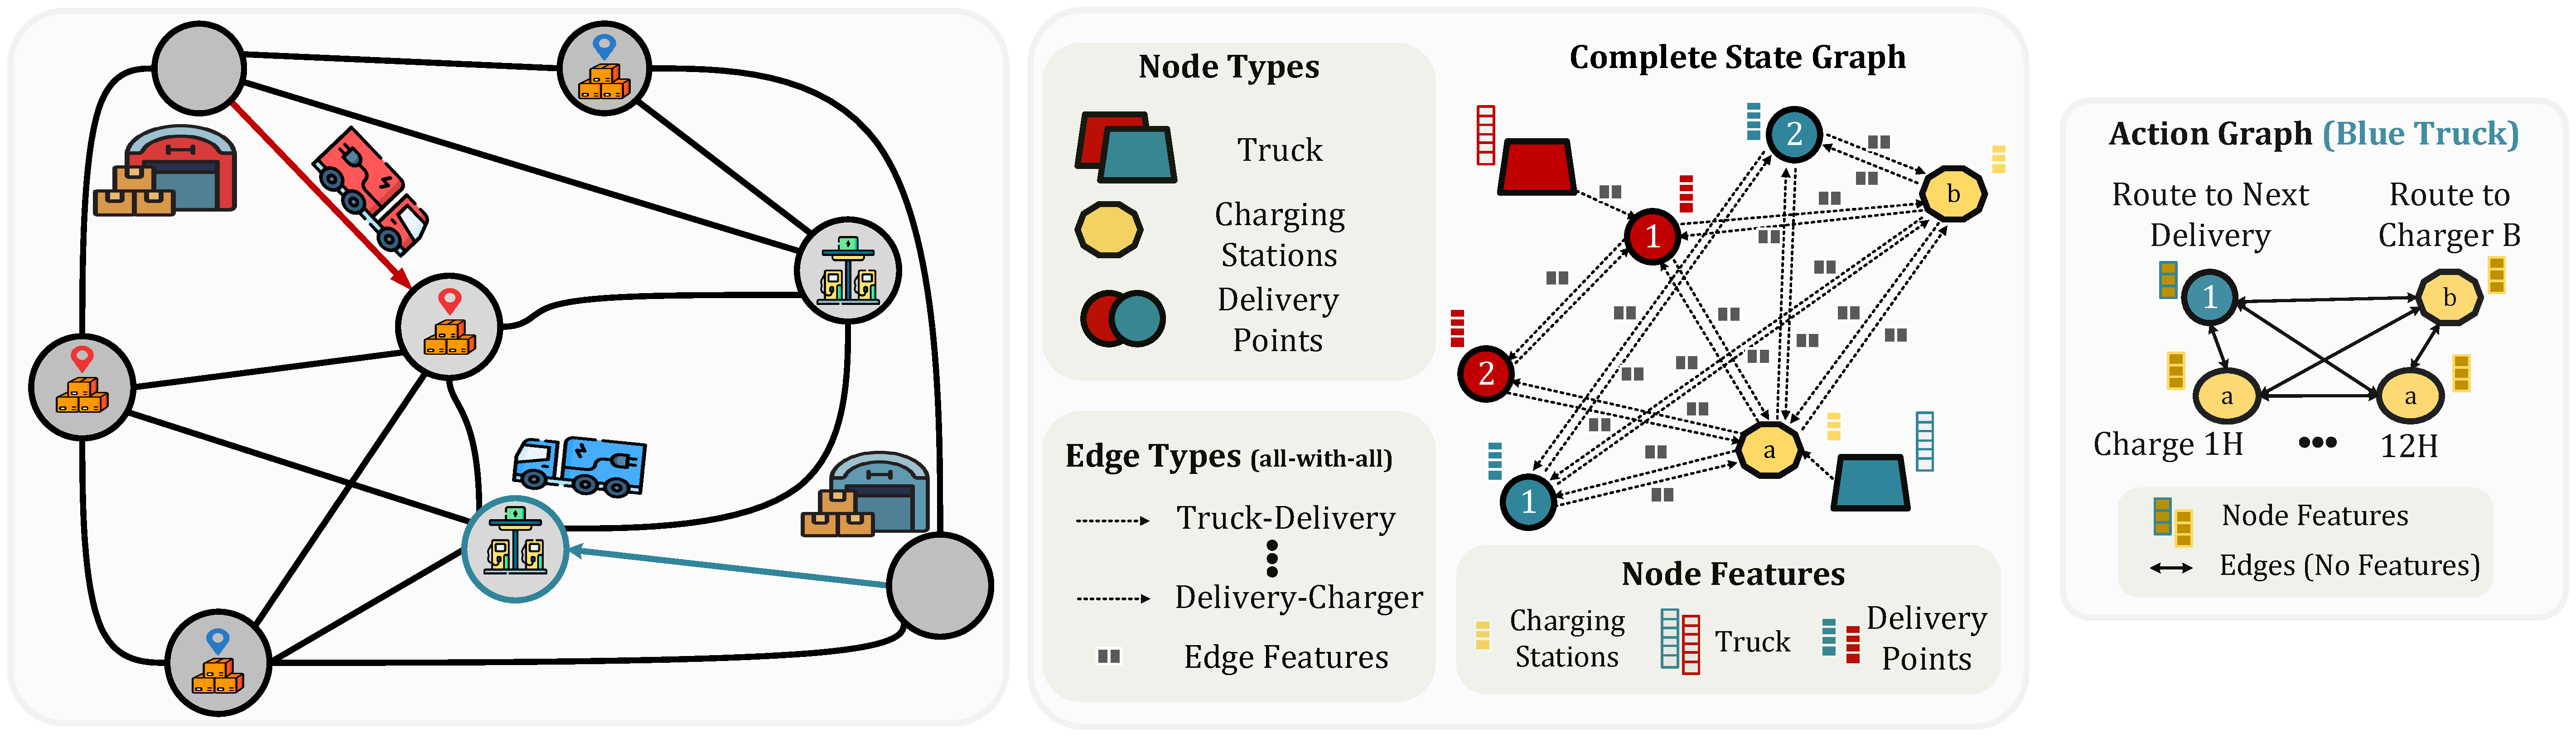
\includegraphics[width=0.98\linewidth]{TruckGraph.pdf}
    % \caption{Illustration of the process of turning the problem state at a step to a state and action graph, by converting objects to distinct nodes, e.g., trucks, chargers, deliveries.}
    \caption{Illustration of the graph construction process at a decision step. The current system state is transformed into a heterogeneous state graph by representing trucks, charging stations, and delivery locations as distinct node types, while feasible routing and charging decisions are encoded in a corresponding action graph.}
    \label{fig:graph_conv}
\end{figure}




\subsection{Graph-Based Semi Markov Decision Process}\label{sec:smdp}
The eTFRP operates in continuous time, and decisions are requested only when a truck enters the \texttt{Action\_Pending} state. Because decision steps are not separated by fixed time intervals, this yields an SMDP~\cite{Elsevier2013_ISBN9780124077959} defined by the tuple
$\big(\mathcal{S},\{\mathcal{A}(s)\}_{s\in\mathcal{S}},P,r,\gamma\big)$,
where $s_t\in\mathcal{S}$ denotes the state observed at the $t$-th decision step, $\mathcal{A}(s_t)$ is the state dependent action space, $P$ is a transition kernel that governs both the next state and the holding time between decisions, $r$ is the reward, and $\gamma\in(0,1)$ is a discount factor. 
% Let $\{g_t\}_{t\ge 0}$ denote the increasing sequence of global times at which decision epochs occur (i.e., \textsc{TRUCK\_READY} events in the event-driven simulator), and define the random holding time $\Delta t_t \triangleq g_{t+1}-g_t$.
The transition kernel $P(s_{t+1} \mid s_t, a_t)$ is determined by the event-driven dynamics of~\eqref{eq:con_battery_bounds}--\eqref{eq:con_ports}: after action $a_t$ is taken at state $s_t$, the simulator advances time to the next event and returns $s_{t+1}$. 

\subsubsection{The state space}

At each decision step $t$ only a single truck becomes active; if several are ready at the same time, one is selected at random. Besides the active truck, the state contains the full system state needed to evaluate feasibility and simulate subsequent evolution. The state $s_t\in \mathcal{S}$ is represented as a heterogeneous graph $\mathcal{G}^{\mathcal{S}}_t(\mathcal{V}^{\mathcal{S}}_t,\mathcal{E}^{\mathcal{S}}_t) \subset \mathcal{G}(\mathcal{V},\mathcal{E})$ built on the same entities and symbols used in the problem formulation described in Section~\ref{sec:problem_definition}.
Specifically, as illustrated in Figure~\ref{fig:graph_conv}, a snapshot of the whole eTFRP system state can be converted into the state graph $\mathcal{G}^{\mathcal{S}}_t$ containing three node types comprising the node set $\mathcal{V}^{\mathcal{S}}_t$. Truck nodes are indexed by $i\in\mathcal{I}$, delivery nodes indexed by $d\in\mathcal{D}$, and charging-station nodes indexed by $c\in\mathcal{C}$.

Each truck node has a feature vector $x^{\mathrm{Truck}}_i(t)\in\mathbb{R}$ defined as
\begin{equation}
x^{\mathrm{Truck}}_i(t)=
\Big[
\tfrac{b_i(t)}{\overline{b}_i},
\text{status}_i(t),
\tfrac{|\mathcal{D}^*_i(t)|}{K_i},
\tfrac{t_i^{\text{elapsed}}(t)}{T},
\tfrac{t_i^{\text{arrival}}(t)}{T}
\Big]^\top\!\!,
\label{eq:truck_features}
\end{equation}
where the first term is the SoC of the truck, the second term denotes the operational status of truck $i$ in the event-driven simulator with a normalized one-hot encoding (e.g., \texttt{ready}, \texttt{routing}, \texttt{charging}, \texttt{waiting\_to\_charge}, \texttt{unloading}).
The set $|\mathcal{D}^*_i(t)| \in \{1,\dots, {K_i}\}$ denotes the number of remaining deliveries for truck $i$, while $K_i$ is the total number of deliveries; hence, the third term is the normalized number of remaining deliveries. The scalar $t_i^{\text{elapsed}}(t)$ denotes the elapsed time since the start of truck $i$'s episode (normalized by the maximum simulation time $T$).
% and $d_i^{\text{traveled}}(t)$ denotes the cumulative distance traveled.
Finally, $t_i^{\text{arrival}}(t)$ shows the estimation of the next ``Action Pending'' event of truck $i$, so it would be zero for the active truck. 

Each pending delivery node for truck $i$ at step $t$ ($d\in\mathcal{D}^*_i(t) \subseteq \mathcal{D}_i$) carries the feature vector $x^{\mathrm{Delivery}}_d(t)=[\,d_{i,k},\,|\mathcal{D}^{*}_{i}(t)|\,]^\top$. Already completed deliveries are not included as nodes, as they no longer affect future decisions.

Finally, each charging-station node $c\in\mathcal{C}$ has a feature vector defined as:
\begin{equation}
x^{\mathrm{Charger}}_c(t)\;=\;
\Big[
c,
\overline{p}_c,\;
\eta_c,\;
\kappa_c,\;
\frac{|\mathcal{M}_c(t)|}{\kappa_c},\;
q_c(t)
\Big]^\top,
\forall c \in \mathcal{C}
\label{eq:charger_features}
\end{equation}
 where $q_c(t)$ is the queue length at station $c$ and the remaining symbols are as defined in Section~\ref{sec:problem_definition}. Charging prices are assumed homogeneous across the network and are therefore excluded.

The edges $\mathcal{E}_t$ of the graph are designed to reflect the transportation costs between all available nodes, as shown in the state graph of Figure~\ref{fig:graph_conv}.
Edges are constructed for each pair of nodes $v,u\in\mathcal{C}\cup\mathcal{D}^*(t)\cup\mathcal{I}$, with features $x^{\mathrm{Edge}}_{uv}(t)=[\tau_{uv},\, e_{uv}]^\top$.
% using the base travel time $\tau_{uv}$ and base energy requirement $e_{uv}$ defined on the directed graph $G=(\mathcal{V},\mathcal{E})$. 
Since $\mathcal{G}$ is not assumed symmetric, these edge features generally satisfy $x^{\mathrm{edge}}_{uv}(t)\neq x^{\mathrm{edge}}_{vu}(t)$ when reversing direction, capturing direction-dependent travel and energy costs.

\subsubsection{The feasible action space}\label{sec:feasible_actions}

The action space is state-dependent: at each decision step only a subset of routing and charging decisions is feasible, given the active truck's location and battery energy, the remaining deliveries, and the instantaneous availability of charging ports. 

To reduce the number of action combinations, navigation to chargers is screened by detour. Let $\bar{d}_{i}(t)$ be a reference delivery, defined as $\bar{d}_{i}(t)=d_{i}^{k_{i}(t)+1}$ in sequential mode and as the closest remaining delivery in flexible mode. For each station $c\in\mathcal{C}$, the incremental detour in nominal travel time of visiting $c$ before continuing toward $\bar{d}_{i_t}(t)$ is
\begin{equation}
\Delta \tau _{i,c} \;=\;\tau_{n_{i}(t),c}+\tau_{c,\bar{d}_{i}(t)}-\tau_{n_{i}(t),\bar{d}_{i}(t)}.
\label{eq:charger_detour}
\end{equation}
Only the $k^{\mathrm{chg}}$ chargers with the smallest detour durations are retained as candidates.
The resulting set of candidate navigation destinations is then
$\hat{\mathcal{V}}_{t}:\{\mathcal{C}^{K_{\mathrm{chg}}}_{i}(t)\ \cup\ \mathcal{D}^{*}_{i}(t)$\}.

Furthermore, a navigation decision to $v\in\hat{\mathcal{V}}_{t}$ is feasible only if it satisfies the conservative energy condition introduced in~\eqref{eq:con_energy_headroom}. This yields the feasible navigation action set
\begin{equation}
\mathcal{A}^{\mathrm{nav}}(s_t)\;=\;\Big\{\;\text{navigate}(v)\;:\; v\in \hat{\mathcal{V}}_{t},\ \alpha\,e_{n_{i}(t),v}<b_{i}(t)\;\Big\},
\label{eq:feasible_nav}
\end{equation}
which filters candidate destinations by requiring sufficient battery energy under the safety multiplier $\alpha\ge 1$.

Charging decisions are meaningful only when the active truck is at a station with a free port. When $n_i(t)=c\in\mathcal{C}$ and a port is available, the truck may select a charging duration $h$ from the discrete set $\mathcal{H}=\{1,2,\ldots,12\}$ (hours), since a truck should not require more than 12 hours to fully charge on fast chargers. The feasible charging actions are therefore
\begin{equation}
\begin{split}
\mathcal{A}^{\mathrm{chg}}(s_t)=\big\{\text{charge}(c,h): \; & c=n_{i}(t)\in\mathcal{C},\\
& |\mathcal{M}_c(t)|<\kappa_c,\ h\in\mathcal{H}\big\}.
\end{split}
\label{eq:feasible_charge}
\end{equation}
The overall feasible action set at step $t$ is given by
$\mathcal{A}(s_t)\;=\;\mathcal{A}^{\mathrm{nav}}(s_t)\ \cup\ \mathcal{A}^{\mathrm{chg}}(s_t)$,
and can equivalently be represented through a binary feasibility mask $m(s_t)$.

The cardinality of $\mathcal{A}(s_t)$ varies across decision steps. For algorithms that require a fixed action dimension, an upper bound follows from enumerating all navigation and charging-duration actions,
$ \lceil\mathcal{A}\rceil \;=\;|\mathcal{C}| \;+\; |\mathcal{D}_{i}(t)| \;+\; |\mathcal{H}|$,
with infeasible actions suppressed at runtime via the binary mask $m(s_t)$.

As shown in Figure~\ref{fig:graph_conv}, at each step $t$, the action set $\mathcal{A}(s_t)$ is also encoded as an action graph $\mathcal{G}^{\mathcal{A}}_t=(\mathcal{V}^{\mathcal{A}}_t,\mathcal{E}^{\mathcal{A}}_t)$,
where $\mathcal{V}^{\mathcal{A}}_t$ contains one node per feasible action. The graph is fully connected with no edge features since the edges do not have a physical meaning, unlike the state graph, where edges represent physical trip distances. 
Each action node $a$ has a three-dimensional feature vector
\begin{equation}
x^{\text{Action}}(t)=\big[\ \mathrm{type}(a),\ \widehat{b}(a),\ \widehat{t}(a)\ \big]^\top,
\label{eq:action_node_features}
\end{equation}
where $\mathrm{type}(a)$ identifies the action category (navigate-to-delivery, navigate-to-charger, or charge),
$\widehat{b}(a)$ is the estimated battery energy after executing $a$ using the nominal updates in \eqref{eq:con_energy_update_travel}--\eqref{eq:con_energy_update_charge}, and
$\widehat{t}(a)$ is the estimated completion time based on the nominal duration of the routing or charging action. 


\subsubsection{Reward function}\label{sec:reward}
A time-based reward is adopted to align the learning with the eTFRP objective function in~\eqref{eq:obj_time}, while providing additional shaping signals that encourage task completion and discourage unsafe behavior.
The reward is defined as:
\begin{equation}
\begin{split}
r(s_t,a_t,s_{t+1})
=\;& -\lambda_1\,\Delta t_i
+\lambda_2\,\{\text{delivery completed at }t\}\\
&+\lambda_3\,\{\text{failure at }t\},
\end{split}
% -\lambda_1\,\Delta t^{\mathrm{wait}}_i,
\label{eq:reward}
\end{equation}
where $\Delta t_i$ is the time passed since the last ``action pending'' status of truck $i$, comprising the realized travel duration on the selected road-network transition, the realized unloading time, the charging duration, and any waiting incurred in a charger queue.
The reward therefore reflects the operational time consumed by routing, service, and charging decisions under uncertainty. The coefficients satisfy $\lambda_1>0$, $\lambda_2>0$, and $\lambda_3<0$; the delivery term $\lambda_2$ provides a sparse positive signal on each completed delivery, improving exploration.
% In practice, delivery completion is detected when a truck arrives at a non-depot delivery location and finishes the corresponding unloading process, at which point the indicator $\mathbb{I}\{\text{delivery completed at }t\}$ is set to one.
The failure term $\lambda_3$ applies when the battery is depleted en route or the truck is stranded without a feasible continuation, and is large enough to discourage decisions that violate energy feasibility.

\subsection{Graph Actor-Critic Network Architecture}\label{sec:gnn_arch}

\begin{figure}[t]
    \centering
    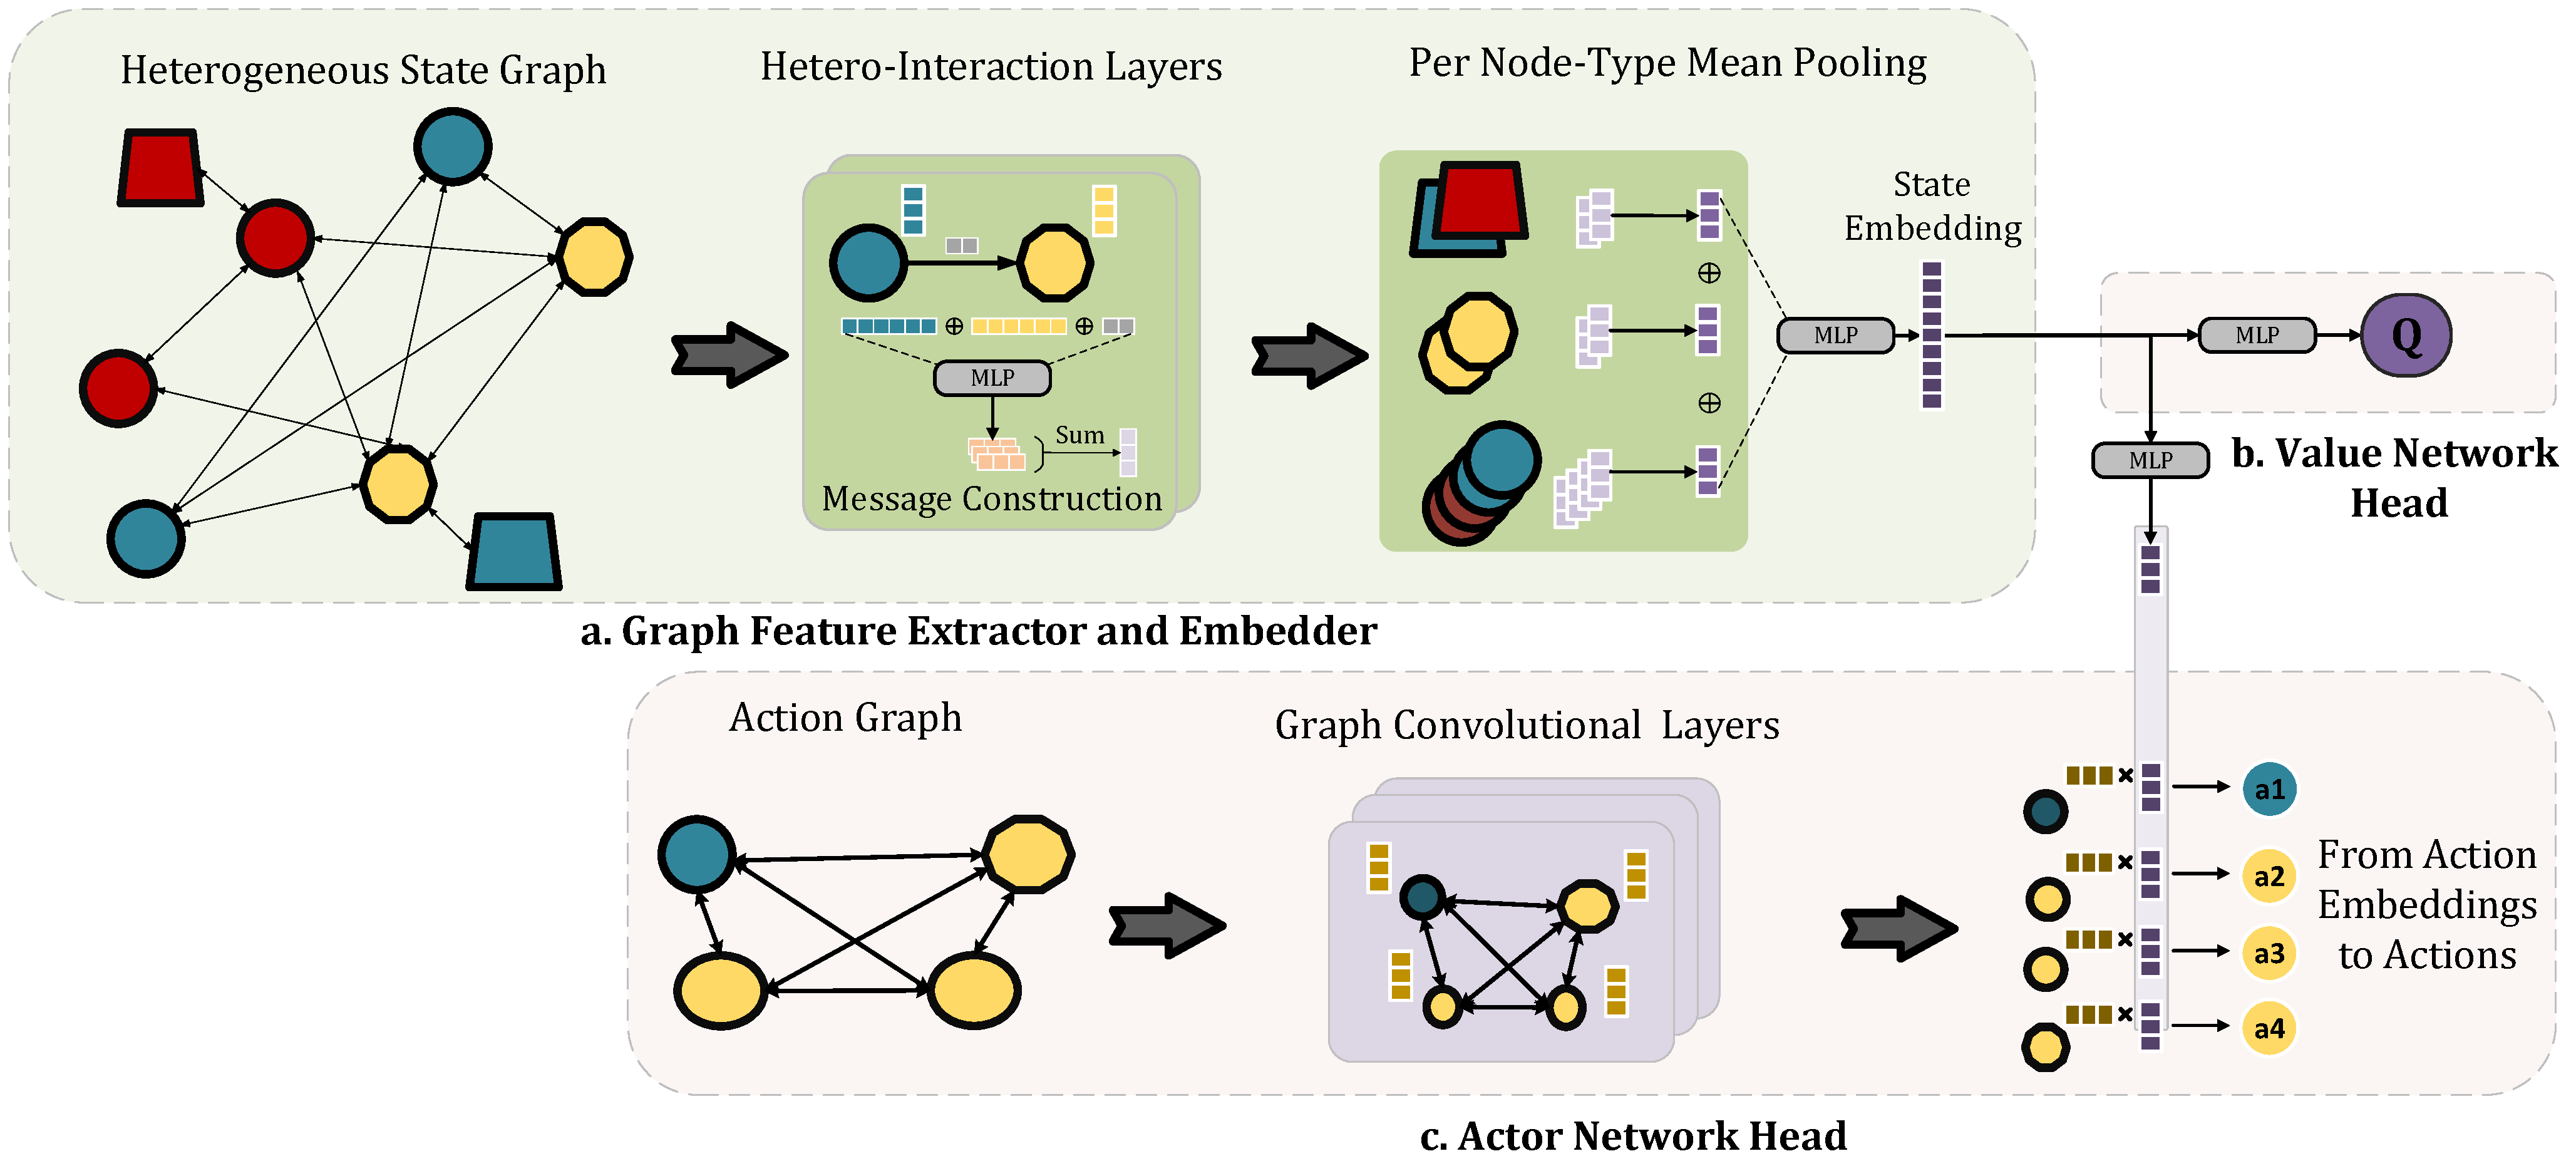
\includegraphics[width=0.72\linewidth]{TruckNetwork.pdf}
    % \caption{The proposed actor-critic neural network that can process the state and action graphs to generate actions and value estimation. }
    \caption{Proposed graph-based actor--critic architecture. In (a), the heterogeneous state graph is encoded through graph feature extraction, hetero-interaction layers~\cite{arowolo2025generalizationgraphneuralnetworks}, and per-node-type mean pooling to obtain a fixed-size global state embedding, invariant to the number of nodes in the state. In (b), the critic head maps this state embedding to a state-value estimate. In (c), the actor head processes the feasible-action graph through graph convolutional layers and combines the resulting action embeddings with the state embedding to produce a policy over routing and charging actions.}
    \label{fig:graph}
\end{figure}


Representing both the state and the feasible action set as graphs yields an actor--critic architecture that exploits the relational structure of the network and the shared charging infrastructure while remaining invariant to the number of trucks, deliveries, and stations. The networks, visualized in Figure~\ref{fig:graph}, consist of a shared heterogeneous graph encoder that maps the state graph $\mathcal{G}^{\mathcal{S}}_t$ to latent representations, followed by (i) an actor head that scores the nodes of the action graph $\mathcal{G}_t^{\mathcal{A}}$ and creates a categorical policy over $\mathcal{A}(s_t)$, and (ii) a critic head that estimates the state value from a state embedding representation of $\mathcal{G}^{\mathcal{S}}_t$.

\subsubsection{State Graph Encoder}

Initially, the heterogeneous state graph $\mathcal{G}^{\mathcal{S}}_t$ is passed through node specific encoders $f_j(x^j)$ producing node embeddings $\{h_j^{(l)}\}$ for each layer $l$ where $j\in\{\mathrm{Truck},\mathrm{Delivery},\mathrm{Charger}\}$ denotes the node type (as defined in Section~\ref{sec:smdp}).
Each node encoder is a single-layer Multilayer Perceptron (MLP) $h_j^{(l)}(x)=W^{(l)}_{j}x+b^{(l)}_{j}$. The node embeddings are then refined through $L$ graph \emph{Hetero-Interaction} layers~\cite{arowolo2025generalizationgraphneuralnetworks}, which perform edge-relation-specific message passing across the directed edges of $\mathcal{G}^\mathcal{S}_t$. 
The edge set $\mathcal{E}^\mathcal{S}_t$ contains several edge types $\mathcal{R}$ (e.g., truck$\rightarrow$delivery, truck$\rightarrow$charger, and their reverses), and $\mathcal{N}_r(v)$ denotes the neighbors of node $v$ under relation $r\in\mathcal{R}$. 
At layer $l\in\{0,\dots,L-1\}$, the messages of the graph convolution operation~\cite{kipf} are computed with a relation-specific affine map applied to the \emph{sender} embedding $h^{(l)}_u$ and the edge feature vector $x^\text{edge}_{uv}$. A message of relation $r$ is then defined as:
\begin{equation}
\mu^{(l)}_{uv,r} \;=\; W^{(l)}_{r} \cdot \big(h_u^{(l)} \; \oplus\; x^\text{edge}_{uv}\big) \;+\;b^{(l)}_{r}.
\label{eq:message}
\end{equation}
% and aggregated per relation,
% \begin{equation}
% \bar{m}^{(l)}_{v,r}
% \;=\;
% \sum_{u\in\mathcal{N}_r(v)} m^{(l)}_{u\rightarrow v,r},
% \label{eq:agg}
% \end{equation}
% where the summation is permutation-invariant over the neighbors of $v$ under relation $r\in\mathcal{R}$.
Messages are averaged over the entire typed neighborhood of $v$, that is over all relations jointly, and the result is combined with the receiver's own embedding through a node-type-specific map, a residual connection, and layer normalization,
\begin{equation}
\begin{split}
\bar{\mu}^{(l)}_{v}
&=
\frac{1}{\max\!\big(1,\textstyle\sum_{r\in\mathcal{R}}|\mathcal{N}_r(v)|\big)}
\sum_{r\in\mathcal{R}}\sum_{u\in\mathcal{N}_r(v)} \mu^{(l)}_{uv,r},\\
h_v^{(l+1)}
&=
\mathrm{LN}\!\Big(
h_v^{(l)} + \sigma\big(U^{(l)}_{\kappa(v)}(h_v^{(l)} \oplus \bar{\mu}^{(l)}_{v})\big)
\Big).
\end{split}
\label{eq:update}
\end{equation}
where $\kappa(v)$ denotes the type of node $v$, $U^{(l)}_{\kappa(v)}$ is the corresponding update matrix, $\mathrm{LN}(\cdot)$ is layer normalization, and $\sigma(\cdot)$ is the Rectified Linear Unit. Directed transportation edges therefore contribute messages that depend on $(\tau_{uv},e_{uv})$, whereas interaction edges between trucks and infrastructure nodes propagate fleet-level context such as station congestion.

Finally, as shown in Figure~\ref{fig:graph}.a, the global state embedding $z_t$ is computed by pooling over the node embeddings. In particular, mean pooling is applied per node type to get the intermediate embeddings $z_{j,t}$.
\begin{equation}
z_{j,t}
=
\frac{1}{\lvert \mathcal{V}^{\mathcal{S}}_{j,t}\rvert}
\sum_{v\in \mathcal{V}_j(\mathcal{G}^{\mathcal{S}}_t)} h_v^{(L)},
\;\; j\in\{\mathrm{Truck},\mathrm{Delivery},\mathrm{Charger}\},
\label{eq:mean_pool_type}
\end{equation}
 Then the intermediate embeddings are concatenated
% \begin{equation}
$z_t \;=\; z_{\mathrm{Truck},t} \;\oplus\; z_{\mathrm{Delivery},t} \;\oplus\; z_{\mathrm{Charger},t}$
% \label{eq:global_pool}
% \end{equation}
to create the final state embedding $z_t$ preserving type information while remaining invariant to the number of nodes in the state graph, such as how many deliveries are left or how many trucks are in the graph.

\subsubsection{Action and Value Function Networks}

As shown in Figure~\ref{fig:graph}.b, the value network maps the state embedding through a fully connected layer, $V_{\phi}(s_t)=\sigma(W_v z_t + b_v)$.
The actor operates on the feasible-action graph $\mathcal{G}_t^\mathcal{A}({\mathcal{V}^\mathcal{A}},\mathcal{E}_t^{\mathcal{A}})$, which holds one node per feasible action and is fully connected with no edge features. As shown in Figure~\ref{fig:graph}.c, each action node is refined via $L^{\mathcal{A}}$ layers of graph convolution. At layer $l\in\{0,\dots,L^{\mathcal{A}}-1\}$, the GCN update for each action node $a$ is
\begin{equation}
\begin{split}
h_{a}^{(l+1)}
= \mathrm{LN}\Big(
h_{a}^{(l)} + \sigma\big(&
W_{\mathrm{self}}^{(l)}h_{a}^{(l)}\\
&+
W_{\mathrm{nbr}}^{(l)}\tfrac{1}{|\mathcal{N}(a)|}\!\!\sum_{v\in\mathcal{N}(a)}\!\! h_{v}^{(l)}
\big)\Big),
\end{split}
\label{eq:action_gcn}
\end{equation}
where $\mathcal{N}(a)=\mathcal{V}^{\mathcal{A}}\setminus\{a\}$ denotes the other feasible actions of the same decision step, so that the aggregation is over \emph{neighboring action embeddings} $h_v^{(l)}$ rather than over the node's own embedding. The mean over neighbors keeps the layer invariant to the number of feasible actions, which varies from step to step, and $\mathrm{LN}(\cdot)$ denotes layer normalization.
Actions are then scored by conditioning the action embeddings on the global state embedding $z_t$ through the dot product $l_t(a) = <h_{a}^{L^{\mathcal{A}}}, z_t>, \; \forall  a\in\mathcal{V}^{\mathcal{A}}$.
The policy is obtained by a softmax over the feasible actions,
\begin{equation}
\pi_{\theta}(a\mid s_t)\;=\;\frac{\exp(l_t(a))}{\sum_{a\in\mathcal{V}^{\mathcal{A}}}\exp(l_t(a))},
\label{eq:actor_policy}
\end{equation}
where $\theta$ is assumed to be all the trainable parameters contributing to the actor network, such as the weights and matrices mentioned before.


Conditioning on the global state embedding~\cite{orfanoudakis2026gnndt} $z_t$ rather than on the active-truck embedding alone lets the policy see system-level interactions such as shared charger occupancy, congestion, and queueing.



\subsection{Variable Action Handling with GraphPPO}\label{sec:ppo}
Here we introduce GraphPPO, outlined in the supplementary material, a PPO~\cite{ppo} variant that uses the graph-based actor--critic architecture of Section~\ref{sec:gnn_arch}.
At each step $t$, the simulator returns the state graph $\mathcal{G}^{\mathcal{S}}_t$ and the feasible action set $\mathcal{A}(s_t)$, from which we build the action graph $\mathcal{G}^{\mathcal{A}}_t$. The actor scores the action nodes to obtain $\pi_\theta(\cdot\mid s_t)$, assigning probability mass only to feasible actions.

Training follows standard PPO: the critic is regressed on one-step Bellman targets, advantages are estimated with generalized advantage estimation, and the actor maximizes the clipped surrogate objective, which constrains the importance ratio to a trust region of width $\epsilon$. The combined loss adds the value regression loss and an entropy bonus to encourage exploration. The objective is stated in full in the supplementary material.






%%%% ==========================================================================================
%%%% ==========================================================================================
%%%% ==========================================================================================






\section{Results}

This section presents the experimental evaluation of the proposed electric truck routing framework. First, the simulation setup is described, including the network configuration, stochastic travel and energy models, charging assumptions, and benchmark settings. The main results are then reported, with emphasis on solution quality, operational feasibility, and computational performance across the tested methods and problem instances.

\subsection{Experimental Setup}



The benchmark is built on a directed transportation network derived from real California road-network data~\cite{ziyan2025}, represented through precomputed shortest-path travel-time and energy dictionaries with charger metadata: 258 candidate delivery nodes, 66{,}049 directed edges, 25 charging stations, and 209 charging ports.
In the main sequential setting, whose random variables and settings are listed in the supplementary material, all vehicles are modeled as homogeneous electric trucks with a battery capacity of 400~kWh, a base speed of 40~km/h, and a full initial state of charge.  At each reset, instances are generated online by assigning each truck a random origin and a feasible ordered delivery sequence satisfying the hop-energy constraints. The charging infrastructure is fixed across instance families, and difficulty is varied through the number of simultaneously operating trucks.

Uncertainty follows Section~\ref{sec:unc}: travel times are Gaussian perturbations of the nominal shortest-path values with rush-hour-dependent variance, realized energy use is correlated with traffic and bounded between 0.90 and 1.20 times nominal while feasibility is checked at the conservative multiplier of 1.20, and charging congestion is endogenous through finite-capacity first-come, first-served stations. Charging decisions are discretized into 12 durations of 1 to 12~h, and energy replenishment follows the CCCV model integrated with a step $\Delta t = 0.01$~h. 

All reported results are averages over 200 evaluation scenarios and 5 training seeds. The evaluation protocol of the joint fleet eVRP study, which uses disjoint seed namespaces and validation-only checkpoint selection, is stated in the supplementary material; differences smaller than the measured cross-seed spread of $0.107$ in success rate are reported as indistinguishable from training noise. GraphPPO's feature extractor has 3 graph layers of 256 nodes, a critic MLP head with 1 layer of 256 nodes, a learning rate of $3\times10^{-4}$, and $\gamma = 0.99$; the nominal training budget for GraphPPO and the PPO-based baselines is $10^6$ environment steps. The PPO and MaskPPO baselines use the default Stable-Baselines3~\cite{sb3} configuration and train in 5--6 hours against about 10 for GraphPPO, on a machine with an A10 GPU, a 16-core Intel CPU, and 24 GB of RAM. 


\subsection{Performance Across Truck Fleet Scales}

Five routing algorithms are compared. Mathematical optimization serves as a high-quality planning reference, obtained by solving the model of Section~\ref{sec:obj_constraints} conservatively under the same environment assumptions but without fully accounting for stochasticity.
The heuristic is a rule-based baseline without learning, generic PPO~\cite{ppo} is applied without any structural adaptation to the transportation graph or the feasibility structure of the problem, and MaskPPO~\cite{maskppo} augments PPO with an action-feasibility mask. GraphPPO extends this through graph-based state and action representations.

Table~\ref{tab:genresults} summarizes eTFRP performance across fleet sizes from 1 truck with 3 stops (1T3S) to 100 trucks (100T3S), evaluated by normalized reward relative to the mathematical benchmark and by the scheduling success rate (routes completed without any stranded trucks); the supplementary material adds the episode-wise ``win ratio'' per scenario. Values slightly above $1.0$ occur because evaluation is stochastic while Math.\ Opt.\ provides a conservative solution. All learning algorithms are trained specifically for each setting.

Table~\ref{tab:genresults} shows a clear separation among methods. GraphPPO is the only learning-based method that retains near-benchmark performance across all settings, with normalized rewards of $0.987$ to $1.005$ and success rates close to Math.\ Opt.\ even at 100 trucks. PPO is very weak throughout, with success falling to $0\%$ from 5T3S onward. MaskPPO shows the strength of the feasible action mask of Section~\ref{sec:feasible_actions} in reward terms, but its robustness degrades sharply with scale, its success declining from $98.0\%$ in 1T3S to $53.0\%$ in 30T3S and $2.0\%$ in 100T3S, and the heuristic reaches $0\%$ success from 30T3S onward.

\label{sec:general-results}
\begin{table*}[t]
\centering
\small
\caption{Performance across eTFRP settings. Each learning-based model was trained for its own setting and evaluated on 200 random scenarios. Entries report normalized reward mean and standard deviation, with the success rate in parentheses (\%); bold marks the best normalized reward per setting.}
\begin{tabular}{@{}lccccc@{}}
\toprule
Setting & Math. Opt. & Heuristic & PPO & MaskPPO & GraphPPO (Ours) \\
\midrule
1T3S & $\mathbf{1.000}$ ($99.5$\%) & $0.806$ $\pm$ $0.448$ ($83.0$\%) & $0.081$ $\pm$ $0.428$ ($15.5$\%) & $0.972$ $\pm$ $0.229$ ($98.0$\%) & $0.987$ $\pm$ $0.136$ ($99.0$\%) \\
5T3S & $\mathbf{1.000}$ ($97.5$\%) & $0.814$ $\pm$ $0.213$ ($42.5$\%) & $0.091$ $\pm$ $0.198$ ($0.0$\%) & $0.980$ $\pm$ $0.085$ ($89.5$\%) & $\mathbf{1.000}$ $\pm$ $0.039$ ($97.0$\%) \\
10T3S & $\mathbf{1.000}$ ($95.5$\%) & $0.803$ $\pm$ $0.150$ ($16.5$\%) & $0.083$ $\pm$ $0.152$ ($0.0$\%) & $0.989$ $\pm$ $0.055$ ($87.5$\%) & $\mathbf{1.000}$ $\pm$ $0.027$ ($95.0$\%) \\
30T3S & $\mathbf{1.000}$ ($88.5$\%) & $0.796$ $\pm$ $0.082$ ($0.0$\%) & $0.125$ $\pm$ $0.086$ ($0.0$\%) & $0.974$ $\pm$ $0.035$ ($53.0$\%) & $0.999$ $\pm$ $0.014$ ($86.5$\%) \\
50T3S & $1.000$ ($77.0$\%) & $0.802$ $\pm$ $0.066$ ($0.0$\%) & $0.305$ $\pm$ $0.090$ ($0.0$\%) & $0.948$ $\pm$ $0.036$ ($4.5$\%) & $\mathbf{1.005}$ $\pm$ $0.013$ ($76.5$\%) \\
100T3S & $1.000$ ($59.5$\%) & $0.800$ $\pm$ $0.048$ ($0.0$\%) & $0.321$ $\pm$ $0.059$ ($0.0$\%) & $0.959$ $\pm$ $0.023$ ($2.0$\%) & $\mathbf{1.005}$ $\pm$ $0.011$ ($60.0$\%) \\
\bottomrule
\end{tabular}
\label{tab:genresults}
\end{table*}

The episode-wise win rates show the same shift. Math.\ Opt.\ wins most scenarios at 10T3S and 30T3S ($54.0\%$ and $55.0\%$, against $26.5\%$ and $43.0\%$ for GraphPPO), whereas in the largest settings GraphPPO attains $84.0\%$ in 50T3S and $78.5\%$ in 100T3S against $15.5\%$ and $21.0\%$: near-benchmark average performance is preserved, and superior competitiveness is achieved in the most congested large-fleet regimes.




Two further eTFRP studies are reported in the supplementary material: a size-transfer analysis of a single policy trained on 100T3S and applied without retraining across fleet sizes and stop counts, and a metric-level breakdown of the 10T3S setting.

\subsection{From eTFRP to Joint Fleet eVRP}\label{sec:joint_evrp}

The preceding subsections assess the eTFRP, in which deliveries are pre-assigned and the fleet competes for shared charging infrastructure. To test whether the proposed representation depends on that structure, a deliberately harder setting restores the decisions the eTFRP removes: customers are owned by the fleet, assignment and sequencing are decided online, payload capacity binds, and every truck must return to the depot. This joint fleet eVRP is solved by the same architecture without modification.

 The objective is total fleet travel time on a plan that serves every customer, and the evaluation is feasibility-first: the success rate dominates and travel time only breaks ties. The optimization benchmark is a fleet-level CP-SAT model over the nominal network with energy-safe repair, whose objective was validated against exhaustive enumeration on tiny instances; an adaptive large neighbourhood search (ALNS) over the same nominal costs is included as a strong metaheuristic and reaches the enumerated optimum wherever enumeration is possible.

\begin{table*}[t]
\centering
\small
\caption{Joint fleet eVRP setting over 500 held-out scenarios, in which assignment, sequencing, charging, and depot return are all decided online. GraphPPO reports the mean over three training seeds with the seed range in brackets; other learning-based rows are single seeds at a smaller interaction budget. Times are fleet totals averaged over all episodes, so a method that declines instances is not flattered by conditioning.}
\begin{tabular}{@{}lcccccc@{}}
\toprule
Metric & CP-SAT & ALNS & Heuristic & PPO & MaskPPO & GraphPPO (Ours) \\
\midrule
Success rate (\%) & $62.2$ & $61.4$ & $55.2$ & $45.2$ & $50.6$ & $\mathbf{84.3}$ $[83.0, 85.8]$ \\
Wilson 95\% CI & $[57.9, 66.3]$ & $[57.1, 65.6]$ & $[50.8, 59.5]$ & $[40.9, 49.6]$ & $[46.2, 55.0]$ & $[79.5, 88.6]$ \\
Completed fraction (-) & $0.932$ & $0.930$ & $0.917$ & $0.960$ & $0.968$ & $\mathbf{0.991}$ \\
Avg.\ truck SoC at finish (\%) & $56$ & $57$ & $62$ & $40$ & $46$ & $49$ \\
Total charging sessions (-) & $34.6$ & $35.4$ & $44.4$ & $16.2$ & $18.9$ & $\mathbf{13.4}$ \\
\midrule
Total charging time (H) & $15.6$ & $15.7$ & $19.4$ & $10.7$ & $11.2$ & $\mathbf{9.4}$ \\
Total routing time (H) & $167.5$ & $168.6$ & $199.8$ & $136.6$ & $143.1$ & $\mathbf{123.5}$ $[120.9, 125.3]$ \\
Unloading time (H) & $1.9$ & $1.9$ & $1.9$ & $2.0$ & $2.0$ & $2.0$ \\
Total time (H) & $184.9$ & $186.3$ & $221.1$ & $149.2$ & $156.3$ & $\mathbf{134.8}$ \\
\midrule
Exec.\ time (ms/decision) & $2.4$ & $2.0$ & $\mathbf{0.8}$ & $1.9$ & $1.9$ & $5.6$ \\
\bottomrule
\end{tabular}
\label{tab:joint_evrp_metrics}
\end{table*}

As shown in Table~\ref{tab:joint_evrp_metrics}, the ordering observed in the eTFRP is preserved when the combinatorial decisions are restored, but the margin is obtained on a different axis.  GraphPPO achieves a success rate of $84.3\%$ against $62.2\%$ for CP-SAT and $61.4\%$ for ALNS, a gap of more than twenty percentage points whose Wilson intervals are disjoint. The two planners agree closely, so their shortfall is not a failure of search but of open-loop execution under realized travel times, energy draws, and service durations.

Because methods decline different instances, a paired reading on jointly solved scenarios is required. On the $285$ scenarios solved by both, GraphPPO and CP-SAT differ by $+0.2$ hours of fleet travel time with a $95\%$ confidence interval of $[-3.1, +3.7]$, and GraphPPO wins $53\%$ of the head-to-head comparisons; against ALNS the difference is $+0.9$ hours $[-2.5, +4.4]$. The proposed method is therefore statistically indistinguishable from a validated exact planner on travel time while completing substantially more instances. Against the remaining baselines the differences are unambiguous: $-23.0$ hours $[-26.7, -19.1]$ against the heuristic and $-26.1$ hours $[-29.7, -22.3]$ against the rolling-horizon controller. Of the learned baselines omitted from the table for width, the strongest is a constructive attention model at $78.8\%$ success and $144.5$ travel hours; at the matched interaction budget it is statistically indistinguishable from the proposed encoder, which is why the state encoder is not claimed as the source of the advantage.

The operational metrics indicate where the advantage originates. The planners build short nominal tours but sustain them with $34.6$ and $35.4$ charging sessions, and they abandon roughly four instances in ten when execution departs from the plan. GraphPPO completes $99.1\%$ of deliveries using $13.4$ charging sessions, and its total operating time of $134.8$ hours is $27\%$ below the planners': a conservative energy policy is retained, but with fewer and better-placed charging stops.

One caveat should be stated plainly: the nominal model here is small enough that CP-SAT proves optimality in milliseconds, so the runtime advantage of the single-vehicle case does not carry over ($5.6$~ms per decision against $2.4$~ms). The argument for the learned policy in this setting rests on solution quality under uncertainty, not on computation time.

\subsection{Ablation and Sensitivity Analysis}\label{sec:ablation}

The joint setting is also used to isolate which components of the proposed representation are responsible for its behaviour, each arm modifying exactly one element while holding the observation width, network shape, interaction budget, curriculum, reward, and seed stream fixed. A component sweep, reported in full in the supplementary material, finds that the per-action routing features, the typed pairwise relations, and the pooled fleet embedding each carry the model, while the charging-queue state and the active-truck indicator are inert on these instances. Because independently seeded runs of the identical configuration span $0.107$ in success rate at this budget, effects smaller than roughly $0.1$ are not separable from training noise.

The feasibility mask, the component most often assumed to explain the performance of masked policies, is examined directly. In a variant where the mask hides only action slots denoting no action at all, so that the policy must learn feasibility from experience, the masked and unmasked variants reach mean success rates of $0.760$ and $0.773$ across three seeds per arm, with overlapping ranges:  at this budget the hard mask is not what produces feasibility. What proves necessary is that infeasibility carry a cost commensurate with failure, as the supplementary material shows; the mask is best understood as a convenience that supplies this cost for free. 

Two further arms, repeating the mask comparison in the pre-assigned variant and varying the charging action space, are reported in the supplementary material; neither changes these conclusions.

\subsection{Transfer Beyond the Training Distribution}\label{sec:transfer}

Transfer is assessed on twenty regimes, each scoring every method on identical held-out scenarios and each labelled as interpolation, size transfer, or genuine distribution shift. Size transfer is strong: success rates of $0.91$, $0.89$, and $0.81$ are obtained at four, six, and eight customers against a ten-customer training distribution, and $0.72$ with a single truck. The ranking is preserved under shifts in charger power and efficiency, port availability, travel-time and energy-draw variance, demand, and road speed, with GraphPPO leading thirteen of the sixteen regimes scored for all methods, usually by more than twenty points.

Three regimes reverse the ranking, and they share a mechanism. With a $300$~kWh battery the learned policy reaches $0.34$ against CP-SAT's $0.43$; with a $500$~kWh battery it reaches $0.87$ against $0.98$; and with service times doubled it reaches $0.46$ against ALNS's $0.60$. Each of these shifts the feasibility frontier itself rather than the cost of an individual decision: a planner re-solves against whatever budget it is given, whereas a policy has internalised where that frontier lies and is miscalibrated when it moves.  Averaged over the out-of-distribution regimes the success rate changes by $-0.110$ for GraphPPO against $-0.006$ for ALNS and $+0.009$ for CP-SAT: the learned policy purchases a large in-distribution advantage and returns part of it where the resource budget changes.

\section{Conclusion}

This paper introduced a truck-oriented, learning-compatible framework for the eTFRP and eVRP under charging constraints, nonlinear charging behavior, and operational uncertainty, formulated as an event-driven semi-Markov decision process and solved with the proposed GraphPPO method.  Across the main multi-truck benchmark, GraphPPO remained close to the mathematical programming baseline, achieving normalized rewards of 0.987--1.005 from 1 to 100 truck instances at success rates near the benchmark's, whereas generic PPO and the heuristics failed almost completely beyond the smallest setting and MaskPPO lost reliability at larger scales. In an additional joint fleet eVRP setting, where assignment, sequencing, and a mandatory depot return were restored as online decisions, the same architecture completed $84.3\%$ of instances against $62.2\%$ for a validated CP-SAT planner while remaining statistically indistinguishable from it on fleet travel time, so the value of the approach extends beyond fleet-level congestion management to the underlying combinatorial routing problem.

Two findings qualify these results and are reported because they bound what the method should be claimed to do. First, an ablation in which the feasibility mask is replaced by one that hides only undefined action slots reaches the same success rate as the masked policy across three training seeds, so the mask is a convenience rather than the source of the reported feasibility; what is necessary is that infeasible actions carry a cost commensurate with failure. Second, transfer holds across instance size and most parameter shifts but degrades where the energy or time budget itself moves, and in those regimes a re-solving planner is the stronger choice.

Future work could extend the benchmark to service constraints such as time windows and depot return policies, and model the routing--charging interaction more deeply through reservation policies, electricity prices, charger heterogeneity, and explicit grid constraints. The degradation observed under shifts of the energy and time budget also suggests that budget-conditioned training, or an explicit feasibility model learned alongside the policy, may be required before such methods can be deployed across heterogeneous fleets without retraining. 

% \section*{Acknowledgements}
% The study was funded by the DriVe2X research and innovation project of the European Commission, grant number 101056934. This work also used the Dutch national e-infrastructure, with support from the SURF Cooperative, under grant no. EINF-5716.

% \printcredits

%% Loading bibliography style file
%\bibliographystyle{model1-num-names}
% \bibliographystyle{cas-model2-names}

%% The two appendices of the Elsevier version (baseline specifications and
%% formulation assumptions) are provided verbatim as supplementary material
%% in supplementary.tex, to keep the main paper within the page limit.

% natbib replaces IEEEtran's own thebibliography, which sets the reference list
% in \footnotesize as the IEEE does; the grouping restores that size.
{\footnotesize
\bibliographystyle{IEEEtranN}
\bibliography{ref}
}

\end{document}
